\documentclass[twoside]{book}

% Packages required by doxygen
\usepackage{fixltx2e}
\usepackage{calc}
\usepackage{doxygen}
\usepackage[export]{adjustbox} % also loads graphicx
\usepackage{graphicx}
\usepackage[utf8]{inputenc}
\usepackage{makeidx}
\usepackage{multicol}
\usepackage{multirow}
\PassOptionsToPackage{warn}{textcomp}
\usepackage{textcomp}
\usepackage[nointegrals]{wasysym}
\usepackage[table]{xcolor}

% Font selection
\usepackage[T1]{fontenc}
\usepackage[scaled=.90]{helvet}
\usepackage{courier}
\usepackage{amssymb}
\usepackage{sectsty}
\renewcommand{\familydefault}{\sfdefault}
\allsectionsfont{%
  \fontseries{bc}\selectfont%
  \color{darkgray}%
}
\renewcommand{\DoxyLabelFont}{%
  \fontseries{bc}\selectfont%
  \color{darkgray}%
}
\newcommand{\+}{\discretionary{\mbox{\scriptsize$\hookleftarrow$}}{}{}}

% Page & text layout
\usepackage{geometry}
\geometry{%
  a4paper,%
  top=2.5cm,%
  bottom=2.5cm,%
  left=2.5cm,%
  right=2.5cm%
}
\tolerance=750
\hfuzz=15pt
\hbadness=750
\setlength{\emergencystretch}{15pt}
\setlength{\parindent}{0cm}
\setlength{\parskip}{3ex plus 2ex minus 2ex}
\makeatletter
\renewcommand{\paragraph}{%
  \@startsection{paragraph}{4}{0ex}{-1.0ex}{1.0ex}{%
    \normalfont\normalsize\bfseries\SS@parafont%
  }%
}
\renewcommand{\subparagraph}{%
  \@startsection{subparagraph}{5}{0ex}{-1.0ex}{1.0ex}{%
    \normalfont\normalsize\bfseries\SS@subparafont%
  }%
}
\makeatother

% Headers & footers
\usepackage{fancyhdr}
\pagestyle{fancyplain}
\fancyhead[LE]{\fancyplain{}{\bfseries\thepage}}
\fancyhead[CE]{\fancyplain{}{}}
\fancyhead[RE]{\fancyplain{}{\bfseries\leftmark}}
\fancyhead[LO]{\fancyplain{}{\bfseries\rightmark}}
\fancyhead[CO]{\fancyplain{}{}}
\fancyhead[RO]{\fancyplain{}{\bfseries\thepage}}
\fancyfoot[LE]{\fancyplain{}{}}
\fancyfoot[CE]{\fancyplain{}{}}
\fancyfoot[RE]{\fancyplain{}{\bfseries\scriptsize Generated by Doxygen }}
\fancyfoot[LO]{\fancyplain{}{\bfseries\scriptsize Generated by Doxygen }}
\fancyfoot[CO]{\fancyplain{}{}}
\fancyfoot[RO]{\fancyplain{}{}}
\renewcommand{\footrulewidth}{0.4pt}
\renewcommand{\chaptermark}[1]{%
  \markboth{#1}{}%
}
\renewcommand{\sectionmark}[1]{%
  \markright{\thesection\ #1}%
}

% Indices & bibliography
\usepackage{natbib}
\usepackage[titles]{tocloft}
\setcounter{tocdepth}{3}
\setcounter{secnumdepth}{5}
\makeindex

% Hyperlinks (required, but should be loaded last)
\usepackage{ifpdf}
\ifpdf
  \usepackage[pdftex,pagebackref=true]{hyperref}
\else
  \usepackage[ps2pdf,pagebackref=true]{hyperref}
\fi
\hypersetup{%
  colorlinks=true,%
  linkcolor=blue,%
  citecolor=blue,%
  unicode%
}

% Custom commands
\newcommand{\clearemptydoublepage}{%
  \newpage{\pagestyle{empty}\cleardoublepage}%
}

\usepackage{caption}
\captionsetup{labelsep=space,justification=centering,font={bf},singlelinecheck=off,skip=4pt,position=top}

%===== C O N T E N T S =====

\begin{document}

% Titlepage & ToC
\hypersetup{pageanchor=false,
             bookmarksnumbered=true,
             pdfencoding=unicode
            }
\pagenumbering{roman}
\begin{titlepage}
\vspace*{7cm}
\begin{center}%
{\Large My Project }\\
\vspace*{1cm}
{\large Generated by Doxygen 1.8.11}\\
\end{center}
\end{titlepage}
\clearemptydoublepage
\tableofcontents
\clearemptydoublepage
\pagenumbering{arabic}
\hypersetup{pageanchor=true}

%--- Begin generated contents ---
\chapter{Class Index}
\section{Class List}
Here are the classes, structs, unions and interfaces with brief descriptions\+:\begin{DoxyCompactList}
\item\contentsline{section}{\hyperlink{structnode}{node} }{\pageref{structnode}}{}
\item\contentsline{section}{\hyperlink{structnode1}{node1} }{\pageref{structnode1}}{}
\item\contentsline{section}{\hyperlink{structnode__info}{node\+\_\+info} }{\pageref{structnode__info}}{}
\end{DoxyCompactList}

\chapter{File Index}
\section{File List}
Here is a list of all files with brief descriptions\+:\begin{DoxyCompactList}
\item\contentsline{section}{\hyperlink{Lab1_8c}{Lab1.\+c} }{\pageref{Lab1_8c}}{}
\end{DoxyCompactList}

\chapter{Class Documentation}
\hypertarget{classAddressBook}{}\section{Address\+Book Class Reference}
\label{classAddressBook}\index{Address\+Book@{Address\+Book}}


{\ttfamily \#include $<$Address\+Book.\+h$>$}

\subsection*{Public Member Functions}
\begin{DoxyCompactItemize}
\item 
\hyperlink{classAddressBook_ad2d2cebd2a3aa00130f769684bc8ddea}{Address\+Book} ()
\item 
\hyperlink{classAddressBook_a5638d9e7361248f33d52894f65597d47}{$\sim$\+Address\+Book} ()
\item 
void \hyperlink{classAddressBook_a55d96137f232d3a52ffb51917d31b32b}{add} ()
\item 
void \hyperlink{classAddressBook_ae4483418575343aa8d53244365a7e475}{search} ()
\item 
void \hyperlink{classAddressBook_ade80a4ffa27ed8a4f9c5c62372d34ea3}{display\+\_\+book} ()
\item 
void \hyperlink{classAddressBook_a524c975a4983e6a0b50f1e89acafa6bb}{edit\+\_\+contact} ()
\item 
void \hyperlink{classAddressBook_a96636dca787ba1a6e3d6ab7b8eb55e45}{delete\+\_\+contact} ()
\item 
void \hyperlink{classAddressBook_a7021de85815ec3aed9d2173fc15faa9b}{sort} ()
\end{DoxyCompactItemize}
\subsection*{Private Attributes}
\begin{DoxyCompactItemize}
\item 
vector$<$ \hyperlink{classContact}{Contact} $\ast$ $>$ \hyperlink{classAddressBook_a2a42a2a0314d0b2c788834caf03b452e}{book}
\end{DoxyCompactItemize}
\subsection*{Friends}
\begin{DoxyCompactItemize}
\item 
void \hyperlink{classAddressBook_ae299771d51ad4ea07d52fbfedb2d6e93}{swap} (int a, int b, vector$<$ \hyperlink{classContact}{Contact} $\ast$ $>$ \&v)
\end{DoxyCompactItemize}


\subsection{Constructor \& Destructor Documentation}
\index{Address\+Book@{Address\+Book}!Address\+Book@{Address\+Book}}
\index{Address\+Book@{Address\+Book}!Address\+Book@{Address\+Book}}
\subsubsection[{\texorpdfstring{Address\+Book()}{AddressBook()}}]{\setlength{\rightskip}{0pt plus 5cm}Address\+Book\+::\+Address\+Book (
\begin{DoxyParamCaption}
{}
\end{DoxyParamCaption}
)}\hypertarget{classAddressBook_ad2d2cebd2a3aa00130f769684bc8ddea}{}\label{classAddressBook_ad2d2cebd2a3aa00130f769684bc8ddea}

\begin{DoxyCode}
21 \{
22    \hyperlink{classContact}{Contact}* c;
23    \textcolor{keywordtype}{char} contact\_type;
24    \hyperlink{AddressBook_8cpp_addb74eb46f4ea2191b74ab5c2a3adb30}{in\_stream}.open(\textcolor{stringliteral}{"AddressBook2.txt"}); \textcolor{comment}{// opens file AddressBook.txt                              
                                                                                                                }
25    \textcolor{keywordflow}{if}(\hyperlink{AddressBook_8cpp_addb74eb46f4ea2191b74ab5c2a3adb30}{in\_stream}.fail()) \textcolor{comment}{// If the file does not open, the program will exit                       
                                                                                                                }
26    \{
27       cout << \textcolor{stringliteral}{"Input file opening failed.\(\backslash\)n"};
28       exit(1);
29    \}
30 
31    \textcolor{keywordflow}{while}(!\hyperlink{AddressBook_8cpp_addb74eb46f4ea2191b74ab5c2a3adb30}{in\_stream}.eof()) \textcolor{comment}{// reads in the values from the file to the end of the file            
                                                                                                                }
32    \{
33       \hyperlink{AddressBook_8cpp_addb74eb46f4ea2191b74ab5c2a3adb30}{in\_stream} >> contact\_type;
34       \textcolor{keywordflow}{if}(contact\_type == \textcolor{charliteral}{'p'})
35       \{
36          c = \textcolor{keyword}{new} \hyperlink{classPersonalContact}{PersonalContact};
37       \}
38       \textcolor{keywordflow}{else} \textcolor{keywordflow}{if}(contact\_type == \textcolor{charliteral}{'b'})
39       \{
40          c = \textcolor{keyword}{new} \hyperlink{classBusinessContact}{BusinessContact};
41       \}
42       c->\hyperlink{classContact_a129d7132ff55adf52737ca7e364d6420}{read}(\hyperlink{AddressBook_8cpp_addb74eb46f4ea2191b74ab5c2a3adb30}{in\_stream});
43       \hyperlink{classAddressBook_a2a42a2a0314d0b2c788834caf03b452e}{book}.push\_back(c);
44    \}
45    \hyperlink{AddressBook_8cpp_addb74eb46f4ea2191b74ab5c2a3adb30}{in\_stream}.close(); \textcolor{comment}{// closes the file                                                          
                                                                                                                }
46    \hyperlink{classAddressBook_a2a42a2a0314d0b2c788834caf03b452e}{book}.pop\_back();
47 \}
\end{DoxyCode}


Here is the call graph for this function\+:
\nopagebreak
\begin{figure}[H]
\begin{center}
\leavevmode
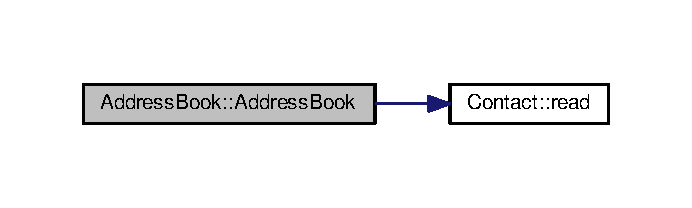
\includegraphics[width=332pt]{classAddressBook_ad2d2cebd2a3aa00130f769684bc8ddea_cgraph}
\end{center}
\end{figure}


\index{Address\+Book@{Address\+Book}!````~Address\+Book@{$\sim$\+Address\+Book}}
\index{````~Address\+Book@{$\sim$\+Address\+Book}!Address\+Book@{Address\+Book}}
\subsubsection[{\texorpdfstring{$\sim$\+Address\+Book()}{~AddressBook()}}]{\setlength{\rightskip}{0pt plus 5cm}Address\+Book\+::$\sim$\+Address\+Book (
\begin{DoxyParamCaption}
{}
\end{DoxyParamCaption}
)}\hypertarget{classAddressBook_a5638d9e7361248f33d52894f65597d47}{}\label{classAddressBook_a5638d9e7361248f33d52894f65597d47}

\begin{DoxyCode}
186 \{
187    \hyperlink{AddressBook_8cpp_a8fb389eff4054f4aa3513963fdaf14a9}{out\_stream}.open(\textcolor{stringliteral}{"AddressBook2.txt"}); \textcolor{comment}{// opens file AddressBook.txt                            
                                                                                                                 }
188    \textcolor{keywordflow}{if}(\hyperlink{AddressBook_8cpp_a8fb389eff4054f4aa3513963fdaf14a9}{out\_stream}.fail()) \textcolor{comment}{// If the file cannot open, the program ends                            
                                                                                                                 }
189    \{
190       cout << \textcolor{stringliteral}{"Output file opening failed.\(\backslash\)n"};
191       exit(1);
192    \}
193 
194    \textcolor{comment}{//for(int k = 0; k < book.size(); k++)                                                                  
                                                                                                       }
195    \textcolor{keywordflow}{for}(vector<Contact*>::iterator it = \hyperlink{classAddressBook_a2a42a2a0314d0b2c788834caf03b452e}{book}.begin(); it != \hyperlink{classAddressBook_a2a42a2a0314d0b2c788834caf03b452e}{book}.end(); it++)
196    \{
197       (*it)->print(\hyperlink{AddressBook_8cpp_a8fb389eff4054f4aa3513963fdaf14a9}{out\_stream}); \textcolor{comment}{// Puts the Contacts from list into the file                     
                                                                                                                 }
198    \}
199    \hyperlink{AddressBook_8cpp_a8fb389eff4054f4aa3513963fdaf14a9}{out\_stream}.close(); \textcolor{comment}{// closes the file                                                        
                                                                                                                 }
200    \textcolor{keywordflow}{for}(\textcolor{keywordtype}{int} k = 0; k < \hyperlink{classAddressBook_a2a42a2a0314d0b2c788834caf03b452e}{book}.size(); k++)
201    \{
202       \textcolor{keyword}{delete} \hyperlink{classAddressBook_a2a42a2a0314d0b2c788834caf03b452e}{book}[k];
203    \}
204 \}
\end{DoxyCode}


\subsection{Member Function Documentation}
\index{Address\+Book@{Address\+Book}!add@{add}}
\index{add@{add}!Address\+Book@{Address\+Book}}
\subsubsection[{\texorpdfstring{add()}{add()}}]{\setlength{\rightskip}{0pt plus 5cm}void Address\+Book\+::add (
\begin{DoxyParamCaption}
{}
\end{DoxyParamCaption}
)}\hypertarget{classAddressBook_a55d96137f232d3a52ffb51917d31b32b}{}\label{classAddressBook_a55d96137f232d3a52ffb51917d31b32b}

\begin{DoxyCode}
50 \{
51    \textcolor{keywordtype}{int} choice = 0;
52    \textcolor{keywordflow}{while}(choice != 1 && choice != 2)
53    \{
54       cout << \textcolor{stringliteral}{"Would you like to create a (1) personal contact, or (2) business contact? "};
55       cin >> choice;
56       \textcolor{keywordflow}{if}(choice != 1 && choice != 2)
57          cout << \textcolor{stringliteral}{"Not a possible choice.\(\backslash\)n"};
58    \}
59 
60    cout << \textcolor{stringliteral}{"Please enter the information for the contact in all six fields:\(\backslash\)n"};
61    cout << \textcolor{stringliteral}{"1. First Name\(\backslash\)n"};
62    cout << \textcolor{stringliteral}{"2. Last Name\(\backslash\)n"};
63    cout << \textcolor{stringliteral}{"3. Telephone Number\(\backslash\)n"};
64    cout << \textcolor{stringliteral}{"4. Date of Birth (mm/dd/yyyy)\(\backslash\)n"};
65    cout << \textcolor{stringliteral}{"5. Email Address\(\backslash\)n"};
66    \textcolor{keywordflow}{if}(choice == 1)
67    \{
68       cout << \textcolor{stringliteral}{"6. Age\(\backslash\)n"};
69       \hyperlink{classContact}{Contact}* pc = \textcolor{keyword}{new} \hyperlink{classPersonalContact}{PersonalContact};
70       pc->\hyperlink{classContact_a129d7132ff55adf52737ca7e364d6420}{read}(cin);
71       \hyperlink{classAddressBook_a2a42a2a0314d0b2c788834caf03b452e}{book}.push\_back(pc);
72    \}
73    \textcolor{keywordflow}{else} \textcolor{keywordflow}{if}(choice == 2)
74    \{
75       cout << \textcolor{stringliteral}{"6. Fax\(\backslash\)n"};
76       \hyperlink{classContact}{Contact}* bc = \textcolor{keyword}{new} \hyperlink{classBusinessContact}{BusinessContact};
77       bc->\hyperlink{classContact_a129d7132ff55adf52737ca7e364d6420}{read}(cin);
78       \hyperlink{classAddressBook_a2a42a2a0314d0b2c788834caf03b452e}{book}.push\_back(bc);
79    \}
80 \}
\end{DoxyCode}


Here is the call graph for this function\+:
\nopagebreak
\begin{figure}[H]
\begin{center}
\leavevmode
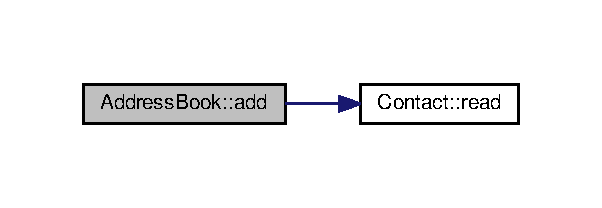
\includegraphics[width=289pt]{classAddressBook_a55d96137f232d3a52ffb51917d31b32b_cgraph}
\end{center}
\end{figure}


\index{Address\+Book@{Address\+Book}!delete\+\_\+contact@{delete\+\_\+contact}}
\index{delete\+\_\+contact@{delete\+\_\+contact}!Address\+Book@{Address\+Book}}
\subsubsection[{\texorpdfstring{delete\+\_\+contact()}{delete_contact()}}]{\setlength{\rightskip}{0pt plus 5cm}void Address\+Book\+::delete\+\_\+contact (
\begin{DoxyParamCaption}
{}
\end{DoxyParamCaption}
)}\hypertarget{classAddressBook_a96636dca787ba1a6e3d6ab7b8eb55e45}{}\label{classAddressBook_a96636dca787ba1a6e3d6ab7b8eb55e45}

\begin{DoxyCode}
114 \{
115    \textcolor{keywordtype}{string} Fname, Lname;
116    cout << \textcolor{stringliteral}{"Enter the first and last names of the contact you would like to delete: "};
117    cin >> Fname >> Lname;
118    cout << endl;
119 
120    \textcolor{keywordflow}{for}(vector<Contact*>::iterator it = \hyperlink{classAddressBook_a2a42a2a0314d0b2c788834caf03b452e}{book}.begin(); it != \hyperlink{classAddressBook_a2a42a2a0314d0b2c788834caf03b452e}{book}.end(); it++)
121    \{
122       \textcolor{keywordflow}{if}((*it)->match(Fname, Lname))
123       \{
124          \hyperlink{classAddressBook_a2a42a2a0314d0b2c788834caf03b452e}{book}.erase(it); \textcolor{comment}{// deletes the Contact from book                                              
                                                                                                           }
125          \textcolor{keywordflow}{return};
126       \}
127    \}
128    cout << \textcolor{stringliteral}{"Contact not found. "} << endl;
129 \}
\end{DoxyCode}
\index{Address\+Book@{Address\+Book}!display\+\_\+book@{display\+\_\+book}}
\index{display\+\_\+book@{display\+\_\+book}!Address\+Book@{Address\+Book}}
\subsubsection[{\texorpdfstring{display\+\_\+book()}{display_book()}}]{\setlength{\rightskip}{0pt plus 5cm}void Address\+Book\+::display\+\_\+book (
\begin{DoxyParamCaption}
{}
\end{DoxyParamCaption}
)}\hypertarget{classAddressBook_ade80a4ffa27ed8a4f9c5c62372d34ea3}{}\label{classAddressBook_ade80a4ffa27ed8a4f9c5c62372d34ea3}

\begin{DoxyCode}
103 \{
104    \textcolor{keywordtype}{int} pnum = 0, bnum = 0;
105    cout << \textcolor{stringliteral}{"-----------------------------------------"} << endl;
106    \textcolor{keywordflow}{for}(vector<Contact*>::iterator it = \hyperlink{classAddressBook_a2a42a2a0314d0b2c788834caf03b452e}{book}.begin(); it != \hyperlink{classAddressBook_a2a42a2a0314d0b2c788834caf03b452e}{book}.end(); it++)\textcolor{comment}{// access all Contact*s
       in book                                                                                                 }
107    \{
108       (*it)->display();
109    \}
110    cout << \textcolor{stringliteral}{"There are "} << \hyperlink{classAddressBook_a2a42a2a0314d0b2c788834caf03b452e}{book}.size() << \textcolor{stringliteral}{" contacts in the address book.\(\backslash\)n"};
111 \}
\end{DoxyCode}
\index{Address\+Book@{Address\+Book}!edit\+\_\+contact@{edit\+\_\+contact}}
\index{edit\+\_\+contact@{edit\+\_\+contact}!Address\+Book@{Address\+Book}}
\subsubsection[{\texorpdfstring{edit\+\_\+contact()}{edit_contact()}}]{\setlength{\rightskip}{0pt plus 5cm}void Address\+Book\+::edit\+\_\+contact (
\begin{DoxyParamCaption}
{}
\end{DoxyParamCaption}
)}\hypertarget{classAddressBook_a524c975a4983e6a0b50f1e89acafa6bb}{}\label{classAddressBook_a524c975a4983e6a0b50f1e89acafa6bb}

\begin{DoxyCode}
132 \{
133    \textcolor{keywordtype}{string} Fname, Lname;
134    cout << \textcolor{stringliteral}{"Enter the first and last names of the contact you would like to edit: "};
135    cin >> Fname >> Lname;
136    cout << endl;
137    \textcolor{keywordflow}{for}(vector<Contact*>::iterator it = \hyperlink{classAddressBook_a2a42a2a0314d0b2c788834caf03b452e}{book}.begin(); it != \hyperlink{classAddressBook_a2a42a2a0314d0b2c788834caf03b452e}{book}.end(); it++)
138    \{
139       \textcolor{keywordflow}{if}((*it)->match(Fname, Lname))
140       \{
141          (*it)->edit(); \textcolor{comment}{// edits the Contact through edit function                                         
                                                                                                       }
142          cout << \textcolor{stringliteral}{"Your edited contact:\(\backslash\)n"} << endl;
143          cout << \textcolor{stringliteral}{"-----------------------------------------"} << endl;
144          (*it)->display(); \textcolor{comment}{// displays the Contact information through display function                    
                                                                                                       }
145          \textcolor{keywordflow}{return};
146       \}
147    \}
148     \hyperlink{classAddressBook_a2a42a2a0314d0b2c788834caf03b452e}{book}[0]->display();
149    cout << \textcolor{stringliteral}{"Contact not found."} << endl;
150 \}
\end{DoxyCode}
\index{Address\+Book@{Address\+Book}!search@{search}}
\index{search@{search}!Address\+Book@{Address\+Book}}
\subsubsection[{\texorpdfstring{search()}{search()}}]{\setlength{\rightskip}{0pt plus 5cm}void Address\+Book\+::search (
\begin{DoxyParamCaption}
{}
\end{DoxyParamCaption}
)}\hypertarget{classAddressBook_ae4483418575343aa8d53244365a7e475}{}\label{classAddressBook_ae4483418575343aa8d53244365a7e475}

\begin{DoxyCode}
83 \{
84    \textcolor{keywordtype}{string} name;
85    cout << \textcolor{stringliteral}{"Please enter a last name to search: "};
86    cin >> name;
87    cout << endl;
88    \textcolor{keywordtype}{int} found = 0;
89    cout << \textcolor{stringliteral}{"-----------------------------------------"} << endl;
90    \textcolor{keywordflow}{for}(vector<Contact*>::iterator it = \hyperlink{classAddressBook_a2a42a2a0314d0b2c788834caf03b452e}{book}.begin(); it != \hyperlink{classAddressBook_a2a42a2a0314d0b2c788834caf03b452e}{book}.end(); it++) \textcolor{comment}{//searches vector book
                                                                                                               }
91    \{
92       \textcolor{keywordflow}{if}((*it)->matchLastName(name)) \textcolor{comment}{// if the last names are the same                                     
                                                                                                       }
93       \{
94          (*it)->display(); \textcolor{comment}{// displays Contact values on screen by calling display function                
                                                                                                       }
95          found++;
96       \}
97    \}
98    \textcolor{keywordflow}{if}(found == 0) \textcolor{comment}{// No Contact was found that has the same last name                                      
                                                                                                       }
99       cout << \textcolor{stringliteral}{"Contact not found. "} << endl;
100 \}
\end{DoxyCode}
\index{Address\+Book@{Address\+Book}!sort@{sort}}
\index{sort@{sort}!Address\+Book@{Address\+Book}}
\subsubsection[{\texorpdfstring{sort()}{sort()}}]{\setlength{\rightskip}{0pt plus 5cm}void Address\+Book\+::sort (
\begin{DoxyParamCaption}
{}
\end{DoxyParamCaption}
)}\hypertarget{classAddressBook_a7021de85815ec3aed9d2173fc15faa9b}{}\label{classAddressBook_a7021de85815ec3aed9d2173fc15faa9b}

\begin{DoxyCode}
160 \{
161    \textcolor{keywordtype}{bool} swaped;
162    \hyperlink{classContact}{Contact} temp;
163    \textcolor{keywordflow}{do}
164    \{
165       swaped = \textcolor{keyword}{false};
166       \textcolor{keywordflow}{for}(\textcolor{keywordtype}{int} k = 0; k < \hyperlink{classAddressBook_a2a42a2a0314d0b2c788834caf03b452e}{book}.size()-1; k++)
167       \{
168          \textcolor{keywordflow}{if}(\hyperlink{classAddressBook_a2a42a2a0314d0b2c788834caf03b452e}{book}[k]->last\_name > \hyperlink{classAddressBook_a2a42a2a0314d0b2c788834caf03b452e}{book}[k+1]->last\_name)
169          \{
170             \hyperlink{classAddressBook_ae299771d51ad4ea07d52fbfedb2d6e93}{swap}(k, k+1, \hyperlink{classAddressBook_a2a42a2a0314d0b2c788834caf03b452e}{book});
171             swaped = \textcolor{keyword}{true};
172          \}
173          \textcolor{keywordflow}{if}(\hyperlink{classAddressBook_a2a42a2a0314d0b2c788834caf03b452e}{book}[k]->last\_name == \hyperlink{classAddressBook_a2a42a2a0314d0b2c788834caf03b452e}{book}[k+1]->last\_name)
174          \{
175             \textcolor{keywordflow}{if}(\hyperlink{classAddressBook_a2a42a2a0314d0b2c788834caf03b452e}{book}[k]->first\_name > \hyperlink{classAddressBook_a2a42a2a0314d0b2c788834caf03b452e}{book}[k+1]->first\_name)
176             \{
177                \hyperlink{classAddressBook_ae299771d51ad4ea07d52fbfedb2d6e93}{swap}(k, k+1, \hyperlink{classAddressBook_a2a42a2a0314d0b2c788834caf03b452e}{book});
178                swaped = \textcolor{keyword}{true};
179             \}
180          \}
181       \}  
182    \}\textcolor{keywordflow}{while}(swaped);
183 \}
\end{DoxyCode}


Here is the call graph for this function\+:
\nopagebreak
\begin{figure}[H]
\begin{center}
\leavevmode
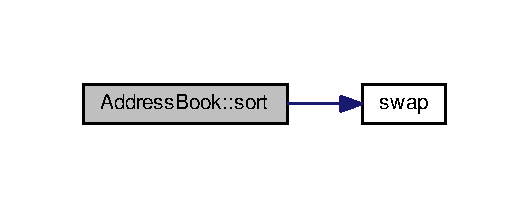
\includegraphics[width=254pt]{classAddressBook_a7021de85815ec3aed9d2173fc15faa9b_cgraph}
\end{center}
\end{figure}




\subsection{Friends And Related Function Documentation}
\index{Address\+Book@{Address\+Book}!swap@{swap}}
\index{swap@{swap}!Address\+Book@{Address\+Book}}
\subsubsection[{\texorpdfstring{swap}{swap}}]{\setlength{\rightskip}{0pt plus 5cm}void swap (
\begin{DoxyParamCaption}
\item[{int}]{a, }
\item[{int}]{b, }
\item[{vector$<$ {\bf Contact} $\ast$ $>$ \&}]{v}
\end{DoxyParamCaption}
)\hspace{0.3cm}{\ttfamily [friend]}}\hypertarget{classAddressBook_ae299771d51ad4ea07d52fbfedb2d6e93}{}\label{classAddressBook_ae299771d51ad4ea07d52fbfedb2d6e93}

\begin{DoxyCode}
153 \{
154    \hyperlink{classContact}{Contact}* temp = v[a];
155    v[a] = v[b];
156    v[b] = temp;
157 \}
\end{DoxyCode}


\subsection{Member Data Documentation}
\index{Address\+Book@{Address\+Book}!book@{book}}
\index{book@{book}!Address\+Book@{Address\+Book}}
\subsubsection[{\texorpdfstring{book}{book}}]{\setlength{\rightskip}{0pt plus 5cm}vector$<${\bf Contact}$\ast$$>$ Address\+Book\+::book\hspace{0.3cm}{\ttfamily [private]}}\hypertarget{classAddressBook_a2a42a2a0314d0b2c788834caf03b452e}{}\label{classAddressBook_a2a42a2a0314d0b2c788834caf03b452e}


The documentation for this class was generated from the following files\+:\begin{DoxyCompactItemize}
\item 
\hyperlink{AddressBook_8h}{Address\+Book.\+h}\item 
\hyperlink{AddressBook_8cpp}{Address\+Book.\+cpp}\end{DoxyCompactItemize}

\hypertarget{classContact}{}\section{Contact Class Reference}
\label{classContact}\index{Contact@{Contact}}
\subsection*{Public Member Functions}
\begin{DoxyCompactItemize}
\item 
\hyperlink{classContact_ac0c3c018b56acb9a064f017a00a3a0c1}{Contact} (string name1, string name2, string date, string number, string e\+\_\+address)
\item 
\hyperlink{classContact_ae39444f378e6de7fd6c3e60981949af5}{Contact} ()
\end{DoxyCompactItemize}
\subsection*{Private Member Functions}
\begin{DoxyCompactItemize}
\item 
void \hyperlink{classContact_a1a7b491fba3111a679bfae344d75d19d}{display} ()
\item 
void \hyperlink{classContact_a1e8e2536913df381990b8ed35d562dd6}{edit} ()
\end{DoxyCompactItemize}
\subsection*{Private Attributes}
\begin{DoxyCompactItemize}
\item 
string \hyperlink{classContact_ac074ba210aa0e4a52921af8353384a59}{first\+\_\+name}
\item 
string \hyperlink{classContact_a87032ae00ab0e8cc81d660f191bcf0fa}{last\+\_\+name}
\item 
string \hyperlink{classContact_a50397132da5dc66f2cb289fc650c3df6}{dob}
\item 
string \hyperlink{classContact_ad23a96ecf0527e8878da50da682ba794}{telephone}
\item 
string \hyperlink{classContact_a7cb8a0ab45d0ddc7a83df39590fcb6c1}{email}
\end{DoxyCompactItemize}
\subsection*{Friends}
\begin{DoxyCompactItemize}
\item 
istream \& \hyperlink{classContact_a83e899a0c8ec90886f1634d7a14e03e2}{operator$>$$>$} (istream \&ins, \hyperlink{classContact}{Contact} \&c)
\item 
ostream \& \hyperlink{classContact_a94e33108c74c0d3b5a4bfd1e1b0ccefa}{operator$<$$<$} (ostream \&outs, const \hyperlink{classContact}{Contact} \&c)
\item 
void \hyperlink{classContact_ac696d2e610fdbff8107ee9710c0d5b15}{add} (vector$<$ \hyperlink{classContact}{Contact} $>$ \&list)
\item 
void \hyperlink{classContact_a216dd5ab87a26c71b6d5b878202dfe82}{search} (vector$<$ \hyperlink{classContact}{Contact} $>$ \&list)
\item 
void \hyperlink{classContact_a7a87b8626d5dde058c954ed4fbbe73c7}{show\+\_\+list} (vector$<$ \hyperlink{classContact}{Contact} $>$ \&list)
\item 
void \hyperlink{classContact_a4ced5629b00075c29878425b2a31afde}{leave} (vector$<$ \hyperlink{classContact}{Contact} $>$ \&list)
\item 
void \hyperlink{classContact_a1a31f84188852ab2b999dd28345d7529}{initialize} (vector$<$ \hyperlink{classContact}{Contact} $>$ \&list)
\item 
void \hyperlink{classContact_a99a4f248002ea076586c3ba4f2ab527d}{edit\+\_\+contact} (vector$<$ \hyperlink{classContact}{Contact} $>$ \&list)
\item 
void \hyperlink{classContact_ace54ad7d307757ff586de3a514eb8357}{delete\+\_\+contact} (vector$<$ \hyperlink{classContact}{Contact} $>$ \&list)
\end{DoxyCompactItemize}


\subsection{Constructor \& Destructor Documentation}
\index{Contact@{Contact}!Contact@{Contact}}
\index{Contact@{Contact}!Contact@{Contact}}
\subsubsection[{\texorpdfstring{Contact(string name1, string name2, string date, string number, string e\+\_\+address)}{Contact(string name1, string name2, string date, string number, string e_address)}}]{\setlength{\rightskip}{0pt plus 5cm}Contact\+::\+Contact (
\begin{DoxyParamCaption}
\item[{string}]{name1, }
\item[{string}]{name2, }
\item[{string}]{date, }
\item[{string}]{number, }
\item[{string}]{e\+\_\+address}
\end{DoxyParamCaption}
)}\hypertarget{classContact_ac0c3c018b56acb9a064f017a00a3a0c1}{}\label{classContact_ac0c3c018b56acb9a064f017a00a3a0c1}

\begin{DoxyCode}
107 \{
108    \hyperlink{classContact_ac074ba210aa0e4a52921af8353384a59}{first\_name} = name1;
109    \hyperlink{classContact_a87032ae00ab0e8cc81d660f191bcf0fa}{last\_name} = name2;
110    \hyperlink{classContact_a50397132da5dc66f2cb289fc650c3df6}{dob} = date;
111    \hyperlink{classContact_ad23a96ecf0527e8878da50da682ba794}{telephone} = number;
112    \hyperlink{classContact_a7cb8a0ab45d0ddc7a83df39590fcb6c1}{email} = e\_address;
113 \}
\end{DoxyCode}
\index{Contact@{Contact}!Contact@{Contact}}
\index{Contact@{Contact}!Contact@{Contact}}
\subsubsection[{\texorpdfstring{Contact()}{Contact()}}]{\setlength{\rightskip}{0pt plus 5cm}Contact\+::\+Contact (
\begin{DoxyParamCaption}
{}
\end{DoxyParamCaption}
)}\hypertarget{classContact_ae39444f378e6de7fd6c3e60981949af5}{}\label{classContact_ae39444f378e6de7fd6c3e60981949af5}

\begin{DoxyCode}
115                 : \hyperlink{classContact_ac074ba210aa0e4a52921af8353384a59}{first\_name}(\textcolor{stringliteral}{""}), \hyperlink{classContact_a87032ae00ab0e8cc81d660f191bcf0fa}{last\_name}(\textcolor{stringliteral}{""}), \hyperlink{classContact_a50397132da5dc66f2cb289fc650c3df6}{dob}(\textcolor{stringliteral}{""}), 
      \hyperlink{classContact_ad23a96ecf0527e8878da50da682ba794}{telephone}(\textcolor{stringliteral}{""}), \hyperlink{classContact_a7cb8a0ab45d0ddc7a83df39590fcb6c1}{email}(\textcolor{stringliteral}{""})
116 \{
117 \}
\end{DoxyCode}


\subsection{Member Function Documentation}
\index{Contact@{Contact}!display@{display}}
\index{display@{display}!Contact@{Contact}}
\subsubsection[{\texorpdfstring{display()}{display()}}]{\setlength{\rightskip}{0pt plus 5cm}void Contact\+::display (
\begin{DoxyParamCaption}
{}
\end{DoxyParamCaption}
)\hspace{0.3cm}{\ttfamily [private]}}\hypertarget{classContact_a1a7b491fba3111a679bfae344d75d19d}{}\label{classContact_a1a7b491fba3111a679bfae344d75d19d}

\begin{DoxyCode}
120 \{
121    cout << \textcolor{stringliteral}{"First Name:       "} << \hyperlink{classContact_ac074ba210aa0e4a52921af8353384a59}{first\_name} << endl;
122    cout << \textcolor{stringliteral}{"Last Name:        "} << \hyperlink{classContact_a87032ae00ab0e8cc81d660f191bcf0fa}{last\_name} << endl;
123    cout << \textcolor{stringliteral}{"Telephone Number: "} << \hyperlink{classContact_ad23a96ecf0527e8878da50da682ba794}{telephone} << endl;
124    cout << \textcolor{stringliteral}{"Date of Birth:    "} << \hyperlink{classContact_a50397132da5dc66f2cb289fc650c3df6}{dob} << endl;
125    cout << \textcolor{stringliteral}{"Email Address:    "} << \hyperlink{classContact_a7cb8a0ab45d0ddc7a83df39590fcb6c1}{email} << endl;
126    cout << \textcolor{stringliteral}{"-----------------------------------------"} << endl;
127 \}
\end{DoxyCode}
\index{Contact@{Contact}!edit@{edit}}
\index{edit@{edit}!Contact@{Contact}}
\subsubsection[{\texorpdfstring{edit()}{edit()}}]{\setlength{\rightskip}{0pt plus 5cm}void Contact\+::edit (
\begin{DoxyParamCaption}
{}
\end{DoxyParamCaption}
)\hspace{0.3cm}{\ttfamily [private]}}\hypertarget{classContact_a1e8e2536913df381990b8ed35d562dd6}{}\label{classContact_a1e8e2536913df381990b8ed35d562dd6}

\begin{DoxyCode}
130 \{
131    \textcolor{keywordtype}{int} choice;
132    \textcolor{keywordflow}{do}
133    \{
134       cout << \textcolor{stringliteral}{"Choose the number of what you would like to edit:\(\backslash\)n"};
135       cout << \textcolor{stringliteral}{"(1) First name\(\backslash\)n"} << \textcolor{stringliteral}{"(2) Last name\(\backslash\)n"} << \textcolor{stringliteral}{"(3) Phone number\(\backslash\)n"} << \textcolor{stringliteral}{"(4) Date of birth\(\backslash\)n"} << \textcolor{stringliteral}{"
      (5) Email address\(\backslash\)n"} << \textcolor{stringliteral}{"(6) Save and finish\(\backslash\)n"};
136       cin >> choice;
137       cout << endl;
138       \textcolor{keywordflow}{switch}(choice) \textcolor{comment}{// checks which choice the user entered                                               
                                                                                                       }
139       \{
140         \textcolor{keywordflow}{case} 1:
141             cout << \textcolor{stringliteral}{"Enter the new first name: "};
142             cin >> \hyperlink{classContact_ac074ba210aa0e4a52921af8353384a59}{first\_name};
143             cout << endl;
144             \textcolor{keywordflow}{break};
145          \textcolor{keywordflow}{case} 2:
146             cout << \textcolor{stringliteral}{"Enter the new last name: "};
147             cin >> \hyperlink{classContact_a87032ae00ab0e8cc81d660f191bcf0fa}{last\_name};
148             cout << endl;
149             \textcolor{keywordflow}{break};
150          \textcolor{keywordflow}{case} 3:
151             cout << \textcolor{stringliteral}{"Enter the new phone number: "};
152             cin >> \hyperlink{classContact_ad23a96ecf0527e8878da50da682ba794}{telephone};
153             cout << endl;
154             \textcolor{keywordflow}{break};
155          \textcolor{keywordflow}{case} 4:
156             cout << \textcolor{stringliteral}{"Enter the new date of birth: "};
157             cin >> \hyperlink{classContact_a50397132da5dc66f2cb289fc650c3df6}{dob};
158             cout << endl;
159             \textcolor{keywordflow}{break};
160          \textcolor{keywordflow}{case} 5:
161             cout << \textcolor{stringliteral}{"Enter the new email address: "};
162             cin >> \hyperlink{classContact_a7cb8a0ab45d0ddc7a83df39590fcb6c1}{email};
163             cout << endl;
164             \textcolor{keywordflow}{break};
165          \textcolor{keywordflow}{case} 6:
166             \textcolor{keywordflow}{return};
167          \textcolor{keywordflow}{default}:
168             cout << \textcolor{stringliteral}{"Not a possible choice.\(\backslash\)n"};
169       \}
170    \}\textcolor{keywordflow}{while} (1);
171 \}
\end{DoxyCode}


\subsection{Friends And Related Function Documentation}
\index{Contact@{Contact}!add@{add}}
\index{add@{add}!Contact@{Contact}}
\subsubsection[{\texorpdfstring{add}{add}}]{\setlength{\rightskip}{0pt plus 5cm}void add (
\begin{DoxyParamCaption}
\item[{vector$<$ {\bf Contact} $>$ \&}]{list}
\end{DoxyParamCaption}
)\hspace{0.3cm}{\ttfamily [friend]}}\hypertarget{classContact_ac696d2e610fdbff8107ee9710c0d5b15}{}\label{classContact_ac696d2e610fdbff8107ee9710c0d5b15}

\begin{DoxyCode}
208 \{
209    \textcolor{keywordtype}{string} f\_name, l\_name, date, number, e\_address;
210    cout << \textcolor{stringliteral}{"Please enter the first name of the entry: "};
211    cin >> f\_name;
212    cout << \textcolor{stringliteral}{"Please enter the last name of the entry: "};
213    cin >> l\_name;
214    cout << \textcolor{stringliteral}{"Please enter the entry's telephone number (put dashes in between): "};
215    cin >> number;
216    cout << \textcolor{stringliteral}{"Please enter the entry's date of birth (mm/dd/yyyy): "};
217    cin >> date;
218    cout << \textcolor{stringliteral}{"Please enter the entry's email address: "};
219    cin >> e\_address;
220    \hyperlink{classContact}{Contact} c(f\_name, l\_name, date, number, e\_address); \textcolor{comment}{// creats Contact c with entered values      
                                                                                                              }
221    list.push\_back(c); \textcolor{comment}{// adds Contact c to vector list                                                     
                                                                                                       }
222 \}
\end{DoxyCode}
\index{Contact@{Contact}!delete\+\_\+contact@{delete\+\_\+contact}}
\index{delete\+\_\+contact@{delete\+\_\+contact}!Contact@{Contact}}
\subsubsection[{\texorpdfstring{delete\+\_\+contact}{delete_contact}}]{\setlength{\rightskip}{0pt plus 5cm}void delete\+\_\+contact (
\begin{DoxyParamCaption}
\item[{vector$<$ {\bf Contact} $>$ \&}]{list}
\end{DoxyParamCaption}
)\hspace{0.3cm}{\ttfamily [friend]}}\hypertarget{classContact_ace54ad7d307757ff586de3a514eb8357}{}\label{classContact_ace54ad7d307757ff586de3a514eb8357}

\begin{DoxyCode}
252 \{
253    \textcolor{keywordtype}{string} Fname, Lname;
254    cout << \textcolor{stringliteral}{"Enter the first and last names of the contact you would like to delete: "};
255    cin >> Fname >> Lname;
256    cout << endl;
257    \textcolor{keywordtype}{int} found = 0;
258    \textcolor{keywordflow}{for}(\textcolor{keywordtype}{int} k = 0; k < list.size(); k++) \textcolor{comment}{// Searches through the vector list                                
                                                                                                       }
259    \{
260       \textcolor{keywordflow}{if}((list[k].\hyperlink{classContact_a87032ae00ab0e8cc81d660f191bcf0fa}{last\_name} == Lname) && (list[k].first\_name == Fname))
261       \{
262          list.erase(list.begin() + k); \textcolor{comment}{// Deletes the Contact from list                                    
                                                                                                       }
263          found++;
264       \}
265    \}
266    \textcolor{keywordflow}{if}(found == 0)
267       cout << \textcolor{stringliteral}{"Contact not found. "} << endl;
268 \}
\end{DoxyCode}
\index{Contact@{Contact}!edit\+\_\+contact@{edit\+\_\+contact}}
\index{edit\+\_\+contact@{edit\+\_\+contact}!Contact@{Contact}}
\subsubsection[{\texorpdfstring{edit\+\_\+contact}{edit_contact}}]{\setlength{\rightskip}{0pt plus 5cm}void edit\+\_\+contact (
\begin{DoxyParamCaption}
\item[{vector$<$ {\bf Contact} $>$ \&}]{list}
\end{DoxyParamCaption}
)\hspace{0.3cm}{\ttfamily [friend]}}\hypertarget{classContact_a99a4f248002ea076586c3ba4f2ab527d}{}\label{classContact_a99a4f248002ea076586c3ba4f2ab527d}

\begin{DoxyCode}
271 \{
272    \textcolor{keywordtype}{string} Fname, Lname;
273    cout << \textcolor{stringliteral}{"Enter the first and last names of the contact you would like to edit: "};
274    cin >> Fname >> Lname;
275    cout << endl;
276    \textcolor{keywordtype}{int} found = 0;
277    \textcolor{keywordflow}{for}(\textcolor{keywordtype}{int} k = 0; k < list.size(); k++)
278    \{
279       \textcolor{keywordflow}{if}((list[k].\hyperlink{classContact_a87032ae00ab0e8cc81d660f191bcf0fa}{last\_name} == Lname) && (list[k].first\_name == Fname))
280       \{
281          list[k].edit(); \textcolor{comment}{// edits the Contact through edit function                                        
                                                                                                       }
282          found++;
283          cout << \textcolor{stringliteral}{"Your edited contact:\(\backslash\)n"} << endl;
284          list[k].display(); \textcolor{comment}{// displays the Contact information through display function                   
                                                                                                       }
285       \}
286    \}
287    \textcolor{keywordflow}{if}(found == 0)
288       cout << \textcolor{stringliteral}{"Contact not found."} << endl;
289 \}
\end{DoxyCode}
\index{Contact@{Contact}!initialize@{initialize}}
\index{initialize@{initialize}!Contact@{Contact}}
\subsubsection[{\texorpdfstring{initialize}{initialize}}]{\setlength{\rightskip}{0pt plus 5cm}void initialize (
\begin{DoxyParamCaption}
\item[{vector$<$ {\bf Contact} $>$ \&}]{list}
\end{DoxyParamCaption}
)\hspace{0.3cm}{\ttfamily [friend]}}\hypertarget{classContact_a1a31f84188852ab2b999dd28345d7529}{}\label{classContact_a1a31f84188852ab2b999dd28345d7529}

\begin{DoxyCode}
190 \{
191    \hyperlink{classContact}{Contact} c;
192    \hyperlink{AddressBook_8cpp_addb74eb46f4ea2191b74ab5c2a3adb30}{in\_stream}.open(\textcolor{stringliteral}{"AddressBook.txt"}); \textcolor{comment}{// opens file AddressBook.txt                               
                                                                                                                }
193    \textcolor{keywordflow}{if}(\hyperlink{AddressBook_8cpp_addb74eb46f4ea2191b74ab5c2a3adb30}{in\_stream}.fail()) \textcolor{comment}{// If the file does not open, the program will exit                       
                                                                                                                }
194    \{
195       cout << \textcolor{stringliteral}{"Input file opening failed.\(\backslash\)n"};
196       exit(1);
197    \}
198 
199    \textcolor{keywordflow}{while}( !\hyperlink{AddressBook_8cpp_addb74eb46f4ea2191b74ab5c2a3adb30}{in\_stream}.eof()) \textcolor{comment}{// reads in the values from the file to the end of the file           
                                                                                                                }
200    \{
201       \hyperlink{AddressBook_8cpp_addb74eb46f4ea2191b74ab5c2a3adb30}{in\_stream} >> c;
202       list.push\_back(c); \textcolor{comment}{// adds Contact c to the vector list                                              
                                                                                                       }
203    \}
204    \hyperlink{AddressBook_8cpp_addb74eb46f4ea2191b74ab5c2a3adb30}{in\_stream}.close(); \textcolor{comment}{// closes the file                                                          
                                                                                                                }
205 \}
\end{DoxyCode}
\index{Contact@{Contact}!leave@{leave}}
\index{leave@{leave}!Contact@{Contact}}
\subsubsection[{\texorpdfstring{leave}{leave}}]{\setlength{\rightskip}{0pt plus 5cm}void leave (
\begin{DoxyParamCaption}
\item[{vector$<$ {\bf Contact} $>$ \&}]{list}
\end{DoxyParamCaption}
)\hspace{0.3cm}{\ttfamily [friend]}}\hypertarget{classContact_a4ced5629b00075c29878425b2a31afde}{}\label{classContact_a4ced5629b00075c29878425b2a31afde}

\begin{DoxyCode}
292 \{
293    \hyperlink{AddressBook_8cpp_a8fb389eff4054f4aa3513963fdaf14a9}{out\_stream}.open(\textcolor{stringliteral}{"AddressBook.txt"}); \textcolor{comment}{// opens file AddressBook.txt                             
                                                                                                                 }
294    \textcolor{keywordflow}{if}(\hyperlink{AddressBook_8cpp_a8fb389eff4054f4aa3513963fdaf14a9}{out\_stream}.fail()) \textcolor{comment}{// If the file cannot open, the program ends                            
                                                                                                                 }
295    \{
296       cout << \textcolor{stringliteral}{"Output file opening failed.\(\backslash\)n"};
297       exit(1);
298    \}
299 
300    \textcolor{keywordflow}{for}(\textcolor{keywordtype}{int} k = 0; k < list.size(); k++)
301    \{
302       \hyperlink{AddressBook_8cpp_a8fb389eff4054f4aa3513963fdaf14a9}{out\_stream} << list[k]; \textcolor{comment}{// Puts the Contacts from list into the file                        
                                                                                                                 }
303    \}
304    \hyperlink{AddressBook_8cpp_a8fb389eff4054f4aa3513963fdaf14a9}{out\_stream}.close(); \textcolor{comment}{// closes the file                                                        
                                                                                                                 }
305    exit(0); \textcolor{comment}{// ends the program                                                                            
                                                                                                       }
306 \}
\end{DoxyCode}
\index{Contact@{Contact}!operator$<$$<$@{operator$<$$<$}}
\index{operator$<$$<$@{operator$<$$<$}!Contact@{Contact}}
\subsubsection[{\texorpdfstring{operator$<$$<$}{operator<<}}]{\setlength{\rightskip}{0pt plus 5cm}ostream\& operator$<$$<$ (
\begin{DoxyParamCaption}
\item[{ostream \&}]{outs, }
\item[{const {\bf Contact} \&}]{c}
\end{DoxyParamCaption}
)\hspace{0.3cm}{\ttfamily [friend]}}\hypertarget{classContact_a94e33108c74c0d3b5a4bfd1e1b0ccefa}{}\label{classContact_a94e33108c74c0d3b5a4bfd1e1b0ccefa}

\begin{DoxyCode}
180 \{
181    outs << c.\hyperlink{classContact_ac074ba210aa0e4a52921af8353384a59}{first\_name} << endl;
182    outs << c.\hyperlink{classContact_a87032ae00ab0e8cc81d660f191bcf0fa}{last\_name} << endl;
183    outs << c.\hyperlink{classContact_a50397132da5dc66f2cb289fc650c3df6}{dob} << endl;
184    outs << c.\hyperlink{classContact_ad23a96ecf0527e8878da50da682ba794}{telephone} << endl;
185    outs << c.\hyperlink{classContact_a7cb8a0ab45d0ddc7a83df39590fcb6c1}{email} << endl;
186    \textcolor{keywordflow}{return} outs;
187 \}
\end{DoxyCode}
\index{Contact@{Contact}!operator$>$$>$@{operator$>$$>$}}
\index{operator$>$$>$@{operator$>$$>$}!Contact@{Contact}}
\subsubsection[{\texorpdfstring{operator$>$$>$}{operator>>}}]{\setlength{\rightskip}{0pt plus 5cm}istream\& operator$>$$>$ (
\begin{DoxyParamCaption}
\item[{istream \&}]{ins, }
\item[{{\bf Contact} \&}]{c}
\end{DoxyParamCaption}
)\hspace{0.3cm}{\ttfamily [friend]}}\hypertarget{classContact_a83e899a0c8ec90886f1634d7a14e03e2}{}\label{classContact_a83e899a0c8ec90886f1634d7a14e03e2}

\begin{DoxyCode}
174 \{
175    ins >> c.\hyperlink{classContact_ac074ba210aa0e4a52921af8353384a59}{first\_name} >> c.\hyperlink{classContact_a87032ae00ab0e8cc81d660f191bcf0fa}{last\_name} >> c.\hyperlink{classContact_a50397132da5dc66f2cb289fc650c3df6}{dob} >> c.
      \hyperlink{classContact_ad23a96ecf0527e8878da50da682ba794}{telephone} >> c.\hyperlink{classContact_a7cb8a0ab45d0ddc7a83df39590fcb6c1}{email};
176    \textcolor{keywordflow}{return} ins;
177 \}
\end{DoxyCode}
\index{Contact@{Contact}!search@{search}}
\index{search@{search}!Contact@{Contact}}
\subsubsection[{\texorpdfstring{search}{search}}]{\setlength{\rightskip}{0pt plus 5cm}void search (
\begin{DoxyParamCaption}
\item[{vector$<$ {\bf Contact} $>$ \&}]{list}
\end{DoxyParamCaption}
)\hspace{0.3cm}{\ttfamily [friend]}}\hypertarget{classContact_a216dd5ab87a26c71b6d5b878202dfe82}{}\label{classContact_a216dd5ab87a26c71b6d5b878202dfe82}

\begin{DoxyCode}
225 \{
226    \textcolor{keywordtype}{string} name;
227    cout << \textcolor{stringliteral}{"Please enter a last name to search: "};
228    cin >> name;
229    cout << endl;
230    \textcolor{keywordtype}{int} found = 0;
231    \textcolor{keywordflow}{for}(\textcolor{keywordtype}{int} k = 0; k < list.size(); k++) \textcolor{comment}{// searches vector list                                            
                                                                                                       }
232    \{
233       \textcolor{keywordflow}{if}(list[k].\hyperlink{classContact_a87032ae00ab0e8cc81d660f191bcf0fa}{last\_name} == name) \textcolor{comment}{// if the last names are the same                             
                                                                                                                }
234       \{
235          list[k].display(); \textcolor{comment}{// displays Contact values on screen by calling display function               
                                                                                                       }
236          found++;
237       \}
238    \}
239    \textcolor{keywordflow}{if}(found == 0) \textcolor{comment}{// No Contact was found that has the same last name}
240       cout << \textcolor{stringliteral}{"Contact not found. "} << endl;
241 \}
\end{DoxyCode}
\index{Contact@{Contact}!show\+\_\+list@{show\+\_\+list}}
\index{show\+\_\+list@{show\+\_\+list}!Contact@{Contact}}
\subsubsection[{\texorpdfstring{show\+\_\+list}{show_list}}]{\setlength{\rightskip}{0pt plus 5cm}void show\+\_\+list (
\begin{DoxyParamCaption}
\item[{vector$<$ {\bf Contact} $>$ \&}]{list}
\end{DoxyParamCaption}
)\hspace{0.3cm}{\ttfamily [friend]}}\hypertarget{classContact_a7a87b8626d5dde058c954ed4fbbe73c7}{}\label{classContact_a7a87b8626d5dde058c954ed4fbbe73c7}

\begin{DoxyCode}
244 \{
245    \textcolor{keywordflow}{for}(\textcolor{keywordtype}{int} k = 0; k < list.size(); k++) \textcolor{comment}{// access all Contacts in vector list                              
                                                                                                       }
246    \{
247    list[k].display();
248    \}
249 \}
\end{DoxyCode}


\subsection{Member Data Documentation}
\index{Contact@{Contact}!dob@{dob}}
\index{dob@{dob}!Contact@{Contact}}
\subsubsection[{\texorpdfstring{dob}{dob}}]{\setlength{\rightskip}{0pt plus 5cm}string Contact\+::dob\hspace{0.3cm}{\ttfamily [private]}}\hypertarget{classContact_a50397132da5dc66f2cb289fc650c3df6}{}\label{classContact_a50397132da5dc66f2cb289fc650c3df6}
\index{Contact@{Contact}!email@{email}}
\index{email@{email}!Contact@{Contact}}
\subsubsection[{\texorpdfstring{email}{email}}]{\setlength{\rightskip}{0pt plus 5cm}string Contact\+::email\hspace{0.3cm}{\ttfamily [private]}}\hypertarget{classContact_a7cb8a0ab45d0ddc7a83df39590fcb6c1}{}\label{classContact_a7cb8a0ab45d0ddc7a83df39590fcb6c1}
\index{Contact@{Contact}!first\+\_\+name@{first\+\_\+name}}
\index{first\+\_\+name@{first\+\_\+name}!Contact@{Contact}}
\subsubsection[{\texorpdfstring{first\+\_\+name}{first_name}}]{\setlength{\rightskip}{0pt plus 5cm}string Contact\+::first\+\_\+name\hspace{0.3cm}{\ttfamily [private]}}\hypertarget{classContact_ac074ba210aa0e4a52921af8353384a59}{}\label{classContact_ac074ba210aa0e4a52921af8353384a59}
\index{Contact@{Contact}!last\+\_\+name@{last\+\_\+name}}
\index{last\+\_\+name@{last\+\_\+name}!Contact@{Contact}}
\subsubsection[{\texorpdfstring{last\+\_\+name}{last_name}}]{\setlength{\rightskip}{0pt plus 5cm}string Contact\+::last\+\_\+name\hspace{0.3cm}{\ttfamily [private]}}\hypertarget{classContact_a87032ae00ab0e8cc81d660f191bcf0fa}{}\label{classContact_a87032ae00ab0e8cc81d660f191bcf0fa}
\index{Contact@{Contact}!telephone@{telephone}}
\index{telephone@{telephone}!Contact@{Contact}}
\subsubsection[{\texorpdfstring{telephone}{telephone}}]{\setlength{\rightskip}{0pt plus 5cm}string Contact\+::telephone\hspace{0.3cm}{\ttfamily [private]}}\hypertarget{classContact_ad23a96ecf0527e8878da50da682ba794}{}\label{classContact_ad23a96ecf0527e8878da50da682ba794}


The documentation for this class was generated from the following file\+:\begin{DoxyCompactItemize}
\item 
\hyperlink{AddressBook_8cpp}{Address\+Book.\+cpp}\end{DoxyCompactItemize}

\chapter{File Documentation}
\hypertarget{AddressBook2_8cpp}{}\section{Address\+Book2.\+cpp File Reference}
\label{AddressBook2_8cpp}\index{Address\+Book2.\+cpp@{Address\+Book2.\+cpp}}
{\ttfamily \#include $<$iostream$>$}\\*
{\ttfamily \#include $<$string$>$}\\*
{\ttfamily \#include $<$fstream$>$}\\*
{\ttfamily \#include $<$cctype$>$}\\*
{\ttfamily \#include $<$cstdlib$>$}\\*
{\ttfamily \#include $<$vector$>$}\\*
Include dependency graph for Address\+Book2.\+cpp\+:
\nopagebreak
\begin{figure}[H]
\begin{center}
\leavevmode
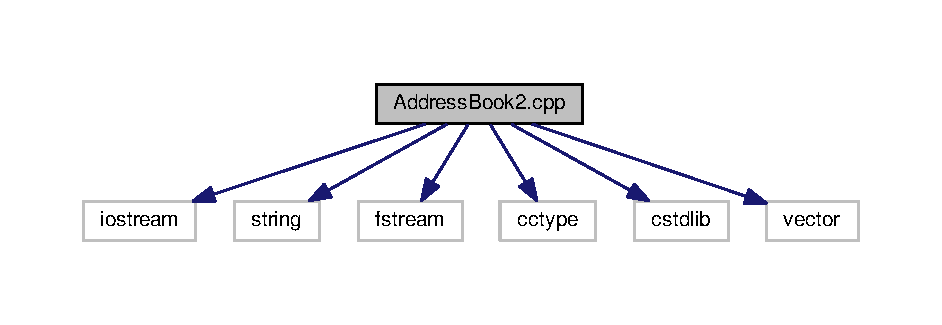
\includegraphics[width=350pt]{AddressBook2_8cpp__incl}
\end{center}
\end{figure}
\subsection*{Classes}
\begin{DoxyCompactItemize}
\item 
class \hyperlink{classContact}{Contact}
\item 
class \hyperlink{classAddressBook}{Address\+Book}
\end{DoxyCompactItemize}
\subsection*{Functions}
\begin{DoxyCompactItemize}
\item 
int \hyperlink{AddressBook2_8cpp_a05384db5c538ff4331381261c758f897}{get\+\_\+choice} ()
\item 
int \hyperlink{AddressBook2_8cpp_ae66f6b31b5ad750f1fe042a706a4e3d4}{main} ()
\item 
bool \hyperlink{AddressBook2_8cpp_a2f605d15a9e66dc7d58a8370d7a0e6c5}{operator$>$} (\hyperlink{classContact}{Contact} \&a, \hyperlink{classContact}{Contact} \&b)
\item 
bool \hyperlink{AddressBook2_8cpp_a27b54514036a945e7b1e5d70eff7958d}{operator==} (\hyperlink{classContact}{Contact} \&a, \hyperlink{classContact}{Contact} \&b)
\item 
istream \& \hyperlink{AddressBook2_8cpp_a83e899a0c8ec90886f1634d7a14e03e2}{operator$>$$>$} (istream \&ins, \hyperlink{classContact}{Contact} \&c)
\item 
ostream \& \hyperlink{AddressBook2_8cpp_a94e33108c74c0d3b5a4bfd1e1b0ccefa}{operator$<$$<$} (ostream \&outs, const \hyperlink{classContact}{Contact} \&c)
\item 
void \hyperlink{AddressBook2_8cpp_a5cd138fa046f34ab9825f38080786c77}{swap} (int a, int b, vector$<$ \hyperlink{classContact}{Contact} $>$ \&v)
\end{DoxyCompactItemize}
\subsection*{Variables}
\begin{DoxyCompactItemize}
\item 
ifstream \hyperlink{AddressBook2_8cpp_addb74eb46f4ea2191b74ab5c2a3adb30}{in\+\_\+stream}
\item 
ofstream \hyperlink{AddressBook2_8cpp_a8fb389eff4054f4aa3513963fdaf14a9}{out\+\_\+stream}
\end{DoxyCompactItemize}


\subsection{Function Documentation}
\index{Address\+Book2.\+cpp@{Address\+Book2.\+cpp}!get\+\_\+choice@{get\+\_\+choice}}
\index{get\+\_\+choice@{get\+\_\+choice}!Address\+Book2.\+cpp@{Address\+Book2.\+cpp}}
\subsubsection[{\texorpdfstring{get\+\_\+choice()}{get_choice()}}]{\setlength{\rightskip}{0pt plus 5cm}int get\+\_\+choice (
\begin{DoxyParamCaption}
{}
\end{DoxyParamCaption}
)}\hypertarget{AddressBook2_8cpp_a05384db5c538ff4331381261c758f897}{}\label{AddressBook2_8cpp_a05384db5c538ff4331381261c758f897}

\begin{DoxyCode}
128 \{
129    \textcolor{keywordtype}{int} choice;
130    cout << endl;
131    cout << \textcolor{stringliteral}{"Please choose an option:"} << endl;
132    cout << \textcolor{stringliteral}{"(1) Add a new contact"} << endl;
133    cout << \textcolor{stringliteral}{"(2) Search by last name"} << endl;
134    cout << \textcolor{stringliteral}{"(3) Show the complete list"} << endl;
135    cout << \textcolor{stringliteral}{"(4) Edit a contact"} << endl;
136    cout << \textcolor{stringliteral}{"(5) Delete a contact"} << endl;
137    cout << \textcolor{stringliteral}{"(6) Exit"} << endl;
138    cin >> choice;
139    cout << endl;
140    \textcolor{keywordflow}{return} choice;
141 
142 \}
\end{DoxyCode}
\index{Address\+Book2.\+cpp@{Address\+Book2.\+cpp}!main@{main}}
\index{main@{main}!Address\+Book2.\+cpp@{Address\+Book2.\+cpp}}
\subsubsection[{\texorpdfstring{main()}{main()}}]{\setlength{\rightskip}{0pt plus 5cm}int main (
\begin{DoxyParamCaption}
{}
\end{DoxyParamCaption}
)}\hypertarget{AddressBook2_8cpp_ae66f6b31b5ad750f1fe042a706a4e3d4}{}\label{AddressBook2_8cpp_ae66f6b31b5ad750f1fe042a706a4e3d4}

\begin{DoxyCode}
94 \{
95    \textcolor{keywordtype}{int} choice;
96    \hyperlink{classAddressBook}{AddressBook} address\_book;
97 
98    cout << endl << \textcolor{stringliteral}{"Welcome to your Address Book!"} << endl;
99    choice = \hyperlink{AddressBook2_8cpp_a05384db5c538ff4331381261c758f897}{get\_choice}();
100    \textcolor{keywordflow}{while}(choice != 6)
101    \{
102       \textcolor{keywordflow}{switch}(choice)
103       \{
104          \textcolor{keywordflow}{case} 1:
105             address\_book.\hyperlink{classAddressBook_a55d96137f232d3a52ffb51917d31b32b}{add}();
106             address\_book.\hyperlink{classAddressBook_a7021de85815ec3aed9d2173fc15faa9b}{sort}();
107             \textcolor{keywordflow}{break};
108          \textcolor{keywordflow}{case} 2:
109             address\_book.\hyperlink{classAddressBook_ae4483418575343aa8d53244365a7e475}{search}();
110             \textcolor{keywordflow}{break};
111          \textcolor{keywordflow}{case} 3:
112             address\_book.\hyperlink{classAddressBook_ade80a4ffa27ed8a4f9c5c62372d34ea3}{display\_book}();
113             \textcolor{keywordflow}{break};
114          \textcolor{keywordflow}{case} 4:
115             address\_book.\hyperlink{classAddressBook_a524c975a4983e6a0b50f1e89acafa6bb}{edit\_contact}();
116             \textcolor{keywordflow}{break};
117          \textcolor{keywordflow}{case} 5:
118             address\_book.\hyperlink{classAddressBook_a96636dca787ba1a6e3d6ab7b8eb55e45}{delete\_contact}();
119             \textcolor{keywordflow}{break};
120         \textcolor{keywordflow}{default}:
121             cout << \textcolor{stringliteral}{"Not a possible choice."} << endl;
122       \}
123       choice = \hyperlink{AddressBook2_8cpp_a05384db5c538ff4331381261c758f897}{get\_choice}();
124    \}
125 \}
\end{DoxyCode}


Here is the call graph for this function\+:
\nopagebreak
\begin{figure}[H]
\begin{center}
\leavevmode
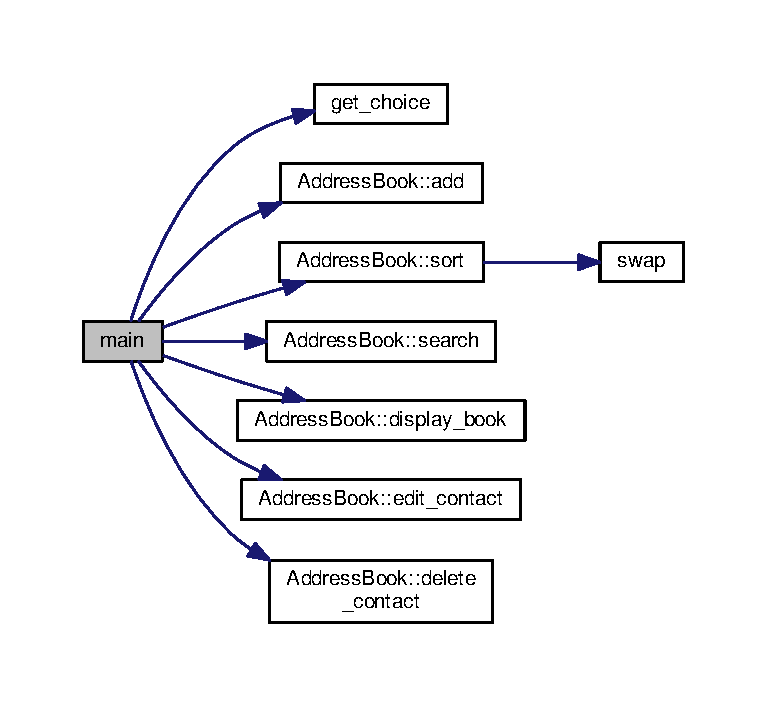
\includegraphics[width=350pt]{AddressBook2_8cpp_ae66f6b31b5ad750f1fe042a706a4e3d4_cgraph}
\end{center}
\end{figure}


\index{Address\+Book2.\+cpp@{Address\+Book2.\+cpp}!operator$<$$<$@{operator$<$$<$}}
\index{operator$<$$<$@{operator$<$$<$}!Address\+Book2.\+cpp@{Address\+Book2.\+cpp}}
\subsubsection[{\texorpdfstring{operator$<$$<$(ostream \&outs, const Contact \&c)}{operator<<(ostream &outs, const Contact &c)}}]{\setlength{\rightskip}{0pt plus 5cm}ostream\& operator$<$$<$ (
\begin{DoxyParamCaption}
\item[{ostream \&}]{outs, }
\item[{const {\bf Contact} \&}]{c}
\end{DoxyParamCaption}
)}\hypertarget{AddressBook2_8cpp_a94e33108c74c0d3b5a4bfd1e1b0ccefa}{}\label{AddressBook2_8cpp_a94e33108c74c0d3b5a4bfd1e1b0ccefa}

\begin{DoxyCode}
265 \{
266    outs << c.\hyperlink{classContact_ac074ba210aa0e4a52921af8353384a59}{first\_name} << endl;
267    outs << c.\hyperlink{classContact_a87032ae00ab0e8cc81d660f191bcf0fa}{last\_name} << endl;
268    outs << c.\hyperlink{classContact_a50397132da5dc66f2cb289fc650c3df6}{dob} << endl;
269    outs << c.\hyperlink{classContact_ad23a96ecf0527e8878da50da682ba794}{telephone} << endl;
270    outs << c.\hyperlink{classContact_a7cb8a0ab45d0ddc7a83df39590fcb6c1}{email} << endl;
271    outs << c.\hyperlink{classContact_a2ff4fdc6afc1afdec2dbfe5cf85f1b92}{fax} << endl;
272    outs << c.\hyperlink{classContact_a68735c7a42c6b9b80ff1b084111e6069}{age} << endl;
273    outs << c.\hyperlink{classContact_ad76971e3edec9fdbc665d149cfbd9e1a}{type} << endl;
274    \textcolor{keywordflow}{return} outs;
275 \}
\end{DoxyCode}
\index{Address\+Book2.\+cpp@{Address\+Book2.\+cpp}!operator==@{operator==}}
\index{operator==@{operator==}!Address\+Book2.\+cpp@{Address\+Book2.\+cpp}}
\subsubsection[{\texorpdfstring{operator==(\+Contact \&a, Contact \&b)}{operator==(Contact &a, Contact &b)}}]{\setlength{\rightskip}{0pt plus 5cm}bool operator== (
\begin{DoxyParamCaption}
\item[{{\bf Contact} \&}]{a, }
\item[{{\bf Contact} \&}]{b}
\end{DoxyParamCaption}
)}\hypertarget{AddressBook2_8cpp_a27b54514036a945e7b1e5d70eff7958d}{}\label{AddressBook2_8cpp_a27b54514036a945e7b1e5d70eff7958d}

\begin{DoxyCode}
254 \{
255    \textcolor{keywordflow}{return} a.\hyperlink{classContact_a87032ae00ab0e8cc81d660f191bcf0fa}{last\_name} == b.\hyperlink{classContact_a87032ae00ab0e8cc81d660f191bcf0fa}{last\_name};
256 \}
\end{DoxyCode}
\index{Address\+Book2.\+cpp@{Address\+Book2.\+cpp}!operator$>$@{operator$>$}}
\index{operator$>$@{operator$>$}!Address\+Book2.\+cpp@{Address\+Book2.\+cpp}}
\subsubsection[{\texorpdfstring{operator$>$(\+Contact \&a, Contact \&b)}{operator>(Contact &a, Contact &b)}}]{\setlength{\rightskip}{0pt plus 5cm}bool operator$>$ (
\begin{DoxyParamCaption}
\item[{{\bf Contact} \&}]{a, }
\item[{{\bf Contact} \&}]{b}
\end{DoxyParamCaption}
)}\hypertarget{AddressBook2_8cpp_a2f605d15a9e66dc7d58a8370d7a0e6c5}{}\label{AddressBook2_8cpp_a2f605d15a9e66dc7d58a8370d7a0e6c5}

\begin{DoxyCode}
249 \{
250    \textcolor{keywordflow}{return} a.\hyperlink{classContact_a87032ae00ab0e8cc81d660f191bcf0fa}{last\_name} > b.\hyperlink{classContact_a87032ae00ab0e8cc81d660f191bcf0fa}{last\_name};
251 \}
\end{DoxyCode}
\index{Address\+Book2.\+cpp@{Address\+Book2.\+cpp}!operator$>$$>$@{operator$>$$>$}}
\index{operator$>$$>$@{operator$>$$>$}!Address\+Book2.\+cpp@{Address\+Book2.\+cpp}}
\subsubsection[{\texorpdfstring{operator$>$$>$(istream \&ins, Contact \&c)}{operator>>(istream &ins, Contact &c)}}]{\setlength{\rightskip}{0pt plus 5cm}istream\& operator$>$$>$ (
\begin{DoxyParamCaption}
\item[{istream \&}]{ins, }
\item[{{\bf Contact} \&}]{c}
\end{DoxyParamCaption}
)}\hypertarget{AddressBook2_8cpp_a83e899a0c8ec90886f1634d7a14e03e2}{}\label{AddressBook2_8cpp_a83e899a0c8ec90886f1634d7a14e03e2}

\begin{DoxyCode}
259 \{
260    ins >> c.\hyperlink{classContact_ac074ba210aa0e4a52921af8353384a59}{first\_name} >> c.\hyperlink{classContact_a87032ae00ab0e8cc81d660f191bcf0fa}{last\_name} >> c.\hyperlink{classContact_a50397132da5dc66f2cb289fc650c3df6}{dob} >> c.
      \hyperlink{classContact_ad23a96ecf0527e8878da50da682ba794}{telephone} >> c.\hyperlink{classContact_a7cb8a0ab45d0ddc7a83df39590fcb6c1}{email} >> c.\hyperlink{classContact_a2ff4fdc6afc1afdec2dbfe5cf85f1b92}{fax} >> c.\hyperlink{classContact_a68735c7a42c6b9b80ff1b084111e6069}{age} >> c.\hyperlink{classContact_ad76971e3edec9fdbc665d149cfbd9e1a}{type};;
261    \textcolor{keywordflow}{return} ins;
262 \}
\end{DoxyCode}
\index{Address\+Book2.\+cpp@{Address\+Book2.\+cpp}!swap@{swap}}
\index{swap@{swap}!Address\+Book2.\+cpp@{Address\+Book2.\+cpp}}
\subsubsection[{\texorpdfstring{swap(int a, int b, vector$<$ Contact $>$ \&v)}{swap(int a, int b, vector< Contact > &v)}}]{\setlength{\rightskip}{0pt plus 5cm}void swap (
\begin{DoxyParamCaption}
\item[{int}]{a, }
\item[{int}]{b, }
\item[{vector$<$ {\bf Contact} $>$ \&}]{v}
\end{DoxyParamCaption}
)}\hypertarget{AddressBook2_8cpp_a5cd138fa046f34ab9825f38080786c77}{}\label{AddressBook2_8cpp_a5cd138fa046f34ab9825f38080786c77}

\begin{DoxyCode}
399 \{
400    \hyperlink{classContact}{Contact} temp = v[a];
401    v[a] = v[b];
402    v[b] = temp;
403 \}
\end{DoxyCode}


\subsection{Variable Documentation}
\index{Address\+Book2.\+cpp@{Address\+Book2.\+cpp}!in\+\_\+stream@{in\+\_\+stream}}
\index{in\+\_\+stream@{in\+\_\+stream}!Address\+Book2.\+cpp@{Address\+Book2.\+cpp}}
\subsubsection[{\texorpdfstring{in\+\_\+stream}{in_stream}}]{\setlength{\rightskip}{0pt plus 5cm}ifstream in\+\_\+stream}\hypertarget{AddressBook2_8cpp_addb74eb46f4ea2191b74ab5c2a3adb30}{}\label{AddressBook2_8cpp_addb74eb46f4ea2191b74ab5c2a3adb30}
\index{Address\+Book2.\+cpp@{Address\+Book2.\+cpp}!out\+\_\+stream@{out\+\_\+stream}}
\index{out\+\_\+stream@{out\+\_\+stream}!Address\+Book2.\+cpp@{Address\+Book2.\+cpp}}
\subsubsection[{\texorpdfstring{out\+\_\+stream}{out_stream}}]{\setlength{\rightskip}{0pt plus 5cm}ofstream out\+\_\+stream}\hypertarget{AddressBook2_8cpp_a8fb389eff4054f4aa3513963fdaf14a9}{}\label{AddressBook2_8cpp_a8fb389eff4054f4aa3513963fdaf14a9}

%--- End generated contents ---

% Index
\backmatter
\newpage
\phantomsection
\clearemptydoublepage
\addcontentsline{toc}{chapter}{Index}
\printindex

\end{document}
